% Using KOMA Script document style
% Font size setting and
% option to skip empty lines as new paragraphs
\documentclass[10pt,a4paper]{article}
% Packages without Options
\usepackage{
	algorithm,
	alltt,
	algpseudocode,
	amsfonts,
	amssymb,
	appendix,
	array,
	booktabs,
	dirtree,
	enumitem,
	float,
	footnote,
	gensymb,
	geometry,
	graphicx,
	interval,
	karnaugh-map,
	lipsum,
	listings,
	longtable,
	makecell,
	mathtools,
	minted,
  nicematrix,
	parskip,
	pdfpages,
	pgfkeys,
	pgfplots,
	subcaption,
	tabularx,
	tablefootnote,
	textcomp,
	tikz,
    titlecaps,
	venndiagram,
	wrapfig,
	wrapfig,
	xcolor
}



% Packages with Options

\usepackage[framemethod=tikz]{mdframed}
\usepackage[colorlinks,linkcolor=cyan, citecolor=cyan, urlcolor=cyan]{hyperref}
\usepackage[labelfont=bf,textfont=it,labelsep=period]{caption}
\usepackage[RPvoltages]{circuitikz}
\usepackage[english]{babel}
\usepackage[nameinlink,noabbrev]{cleveref}

\definecolor{mintedbackground}{rgb}{0.97,0.97,0.97}

\setminted[cpp]{
bgcolor=mintedbackground,
    linenos=true,
    breaklines=true,}

\setminted[js]{
bgcolor=mintedbackground,
    linenos=true,
    breaklines=true,}

\setminted[python]{
bgcolor=mintedbackground,
    linenos=true,
    breaklines=true,}
    

\linespread{1.5}

% Package: AlgorithmicX
% Sets all comments to be indentend and aligned

\renewcommand{\Comment}[2][.7\linewidth]{%
  \leavevmode\hfill\makebox[#1][l]{//~#2}}


% Package: Interval
% Sets the style of mathematical intervals
\intervalconfig{
soft open fences, separator symbol=,,
}

% Package: Geometry
% Sets the page margins
\geometry{
    a4paper,
    left=32mm,
    right=22mm,
    top=22mm,
    }
	
% Creates a proper caption name for algorithms
\newcommand{\algorithmautorefname}{Algorithm}
\newcommand{\listingautorefname}{Listing}
\algrenewcommand{\algorithmiccomment}[1]{\texttt{// #1} }
% Creates a numbered environment for Theorems
\newtheorem{theorem}{Theorem}

% Redefine the implication arrow to be a simple, thin arrow instead of the default, thick arrow
\renewcommand{\implies}{\rightarrow}

% Create a new command for the set complement to make my logical statements easier to read
\newcommand{\compl}{\overline}

% Creates commands for combinatorics nCr and nPr
\newcommand{\nCr}[2]{\,_{#1}C_{#2}} % nCr
\newcommand{\nPr}[2]{\,_{#1}P_{#2}} % nPr

% Package: tikz
% Loads libraries for drawing automata, 
\usetikzlibrary{automata,positioning,shadows,arrows, shapes.gates.logic.US, calc}

% Creates a command to create a button shape
\newcommand*\keystroke[1]{%
  \tikz[baseline= (key.base)]
    \node[%
      draw,
      fill=white,
      drop shadow={shadow xshift=0.25ex,shadow yshift=-0.25ex,fill=black,opacity=0.75},
      rectangle,
      rounded corners=2pt,
      inner sep=1pt,
      line width=0.5pt,
      font=\scriptsize\sffamily
    ] (key) {#1\strut};
}

% Package: pgfplot
% Sets the global options for PGF Plots
\pgfplotsset{compat=newest}

% Package: tikz
% Flowchart Shapes
\tikzstyle{startstop} = [rectangle, rounded corners, minimum width=3cm, minimum height=1cm,text centered, draw=black, fill=red!30]
\tikzstyle{io} = [trapezium, trapezium left angle=70, trapezium right angle=110, minimum width=3cm, minimum height=1cm, text centered, draw=black, fill=blue!30]
\tikzstyle{process} = [rectangle, minimum width=3cm, minimum height=1cm, text centered, draw=black, fill=orange!30]
\tikzstyle{decision} = [diamond, minimum width=3cm, minimum height=1cm, text centered, draw=black, fill=green!30]
\tikzstyle{arrow} = [thick,->,>=stealth]

% Disable Minted syntax error highlights (red boxes)
\AtBeginEnvironment{minted}{%
  \renewcommand{\fcolorbox}[4][]{#4}}

% Listings Style (non-minted)

\lstdefinestyle{arjuncode}{
    basicstyle=\ttfamily,
    breakatwhitespace=false,         
    breaklines=true,                 
    captionpos=b,                    
    keepspaces=true,                 
    numbers=left,                    
    numbersep=5pt,                  
    showspaces=false,                
    showstringspaces=false,
    showtabs=false,                  
    tabsize=2
}

\lstset{style=arjuncode}

\graphicspath{{images/}}


\title{CM2005: Object-Oriented Programming \\ Mid-Term Assignment}
\author{Arjun Muralidharan \\ University of London}
\begin{document}

\maketitle
\newpage
\tableofcontents
\listoffigures
\listoftables
% \listofalgorithms

\newpage
\renewcommand{\subsubsectionautorefname}{section\negthinspace}

\section{General Overview \& Approach}
The objective of this assigment was to develop an automated trading program that emulates the manual operation of the ``Merklerex'' starter application. The application in this submission was largely developed independently from the starter code provided, with some parts copied over to ensure correct basic operation.
The \textbf{key design approach} used in this assignment was to move all core trading logic to a new \texttt{MerkleBot} class, and reducing the original \texttt{MerkleMain} class to only control the user input and output operations. This new relationship is shown in \autoref{fig:merklebot}.
This meant not only creating new functions to address the requirements of the assignment, but also refactoring much of the existing code to use the new class in order to recude duplication.
The bot functionality is invoked as a new, additional menu option of the simulation and can be invoked at the start of the simulation, or after executing one or more manual trades. Once invoked, the rest of the simulation runs in an automated fashion.

\begin{figure}[H]
	\centering
	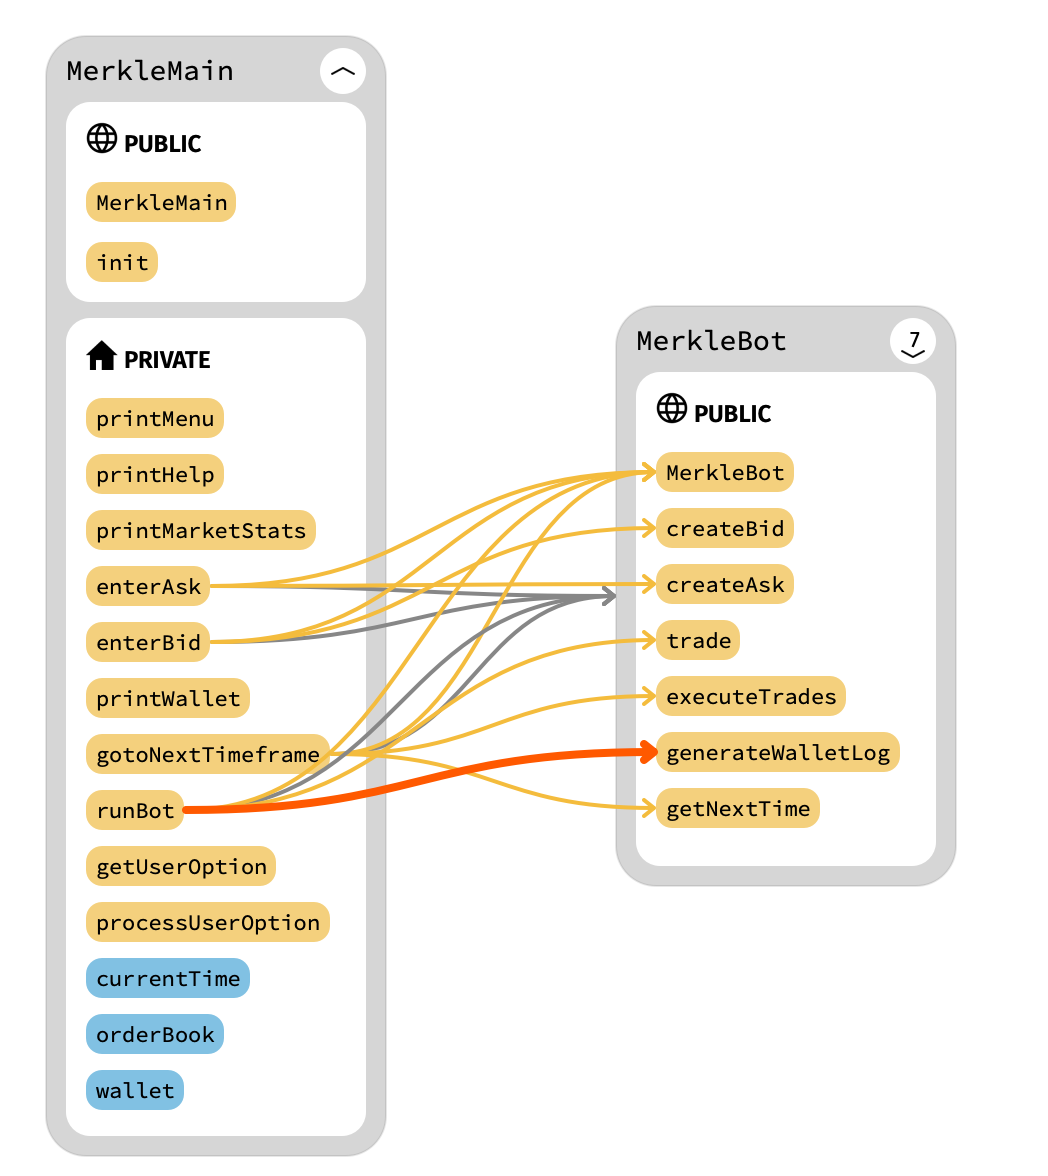
\includegraphics[width=0.7\textwidth]{merklemainbot.png}
	\caption{Relationship between the MerkleMain and MerkleBot classes}
	\label{fig:merklebot}
\end{figure}

\paragraph{Performance considerations} Major refactoring was done to improve performance of the simulation, achieved by using a more efficient data structure to store and operate on the order book data. A \texttt{<map>} structure storing timestamps and their respective orders as a vector yielded significant benefits, as a \texttt{<map>} is stored sorted by keys internally, eliminating the need to sort the order book during the simulation and reducing algorithmic time complexity.

More optimisation is possible by pre-loading and storing frequently used subsets of the market data, however for the scope of this assignment the bot operation was left to operate at between 10 and 30 seconds on typical modern-day CPUs. 

\section{Requirements}
This section describes how each of the requirements were addressed with corresponding code extracts where applicable.
\subsection{R1: Market Analysis}
\subsubsection{R1A: Bot accesses order book}
The bot operates on the same order book as the main application. This is achieved by passing the order book (as well as the wallet and the current time string) as references to the bot at instantiation. As the bot is instantiated, it initialises variables using an initializer list.

This approach, shown in code in \autoref{lis:r1a} allows the bot to be instantiated only when needed, run any required functions which directly operate on the current, most updated versions of the order book (and the wallet), and then the bot can be destroyed safely.

\begin{listing}[H]
	\begin{minted}{cpp}
class MerkleBot
{
public:
	MerkleBot(Wallet& _wallet, OrderBook& _orderBook, std::string& _currentTime);
	Wallet& wallet;
	OrderBook& orderBook;
	std::string& currentTime;
};
\end{minted}

	\begin{minted}{cpp}
MerkleBot::MerkleBot(Wallet& _wallet, OrderBook& _orders, std::string& _currentTime)
	: wallet{_wallet}, orderBook{_orders}, currentTime{_currentTime}
{
}
	\end{minted}
	\caption{Accessing the order book by passing by reference}
	\label{lis:r1a}
\end{listing}

\subsubsection{R1B: Bot can generate predictions of future market prices}

This requirements was achieved by creating an algorithm that generates recommendations of currencies to buy and sell; a type of ``stock picks''. Additionally, a price is picked from the current timeframe at which the currency should be bought or sold.

The algorithm, shown in \autoref{alg:stockpick}, is a largely simplified version of using a \textbf{simple moving average (SMA)} to judge if the price trend of a given currency is positive or negative. If the trend has been negative for a given period of time, this indicates a sell signal. The opposite is true for a buy signal. This is a conservative trading approach relying on trends over a number of timeframes.

\begin{algorithm}[H]
	\caption{Stock Picks Algorithm}
	\begin{algorithmic}
\Function{StockPicks}{}
	\State{predictions \( \leftarrow \)  new Map(OrderBookType, string);}
	\State{buyPredictions \( \leftarrow \) new Map(string, double);}
	\State{sellPredictions  \( \leftarrow \) new Map(string, double);}
\ForAll{product \( \in \)  OrderBook.products}
\If{Simple Moving Average (20 days) \( > \) current high price for asks}
\State{sellPredictions.push(product, current low price for asks)}
\EndIf{}
\If{Simple Moving Average (20 days) \( < \) current high price for bids}
\State{buyPredictions.push(product, current high price for bids)}
\EndIf{}
\EndFor{}
\State{predictions.push(bid, buyPredictions)}
\State{predictions.push(ask, sellPredictions)}
\State{\textbf{return} predictions}
\EndFunction{}

	\end{algorithmic}
\label{alg:stockpick}
\end{algorithm}

The corresponding code is available in the \texttt{StockPicks()} function of the \texttt{MerkleBot} class and reflects the necessary C++ syntax to return a valid map containing two submaps (one each for ask and bid predictions) as a result.

\subsection{R2: Bids, asks and sales}
\subsubsection{R2A: Bot can generate bids and place them in the order book}

The result of the previous \texttt{StockPicks()} function is later called within the \texttt{trade()} function. This function loops through the returned stock picks (using a range-based loop on the map with C++17 structured bindings) and creates bids for each stock pick. The specific code extract responsible for this is shown in \autoref{lis:r2a}.

\begin{listing}[H]
	\begin{minted}{cpp}
void MerkleBot::trade()
{
	// ...
	if (bidPicks.size() > 0)
	{
		for (auto const [product, price] : bidPicks)
		{
			// Get the currency pair for the stock pick product
			std::string currency = product.substr(product.find("/") + 1);

			// Get the correct balance from your wallet
			double balance{wallet.checkBalance(currency)};

			// Create the bid, splitting your balance across all bids for the same currency
			createBid(price, (balance / bidPicks.count(product)) * price, product);
		}
	}
	// ... 
}
	\end{minted}
	\caption{Creating asks and bids based on stock picks}
	\label{lis:r2a}
\end{listing}

The bot has a function called \texttt{createBid} that creates the actual bid. This function has been slightly refactored from the original starter code so it can be used by both the bot as well as manual operation from the \texttt{MerkleMain} class. The code is not reproduced in this document as it is very similar to the starte code and algorithmically unchanged.

\subsubsection{R2B: Bot can generate asks and place them in the order book}
This is solved identically to requirement \emph{R1A}  with the only difference being that the program checks for asks instead of bids.

There is potential to further optimize these procedures so that a single procedure can handle both bids and asks, and the functions \texttt{createBid} and \texttt{createAsk} could be merged to further reduce code duplication.

\subsubsection{R2C: Bot updates wallet after successful sales}
The execution of sales and update to the wallet happens as part of the \texttt{executeTrades} function. This function has been encapsulated to allow for both manual calls from \texttt{MerkleMain} and within the \texttt{trade()} function of the bot.

For each \texttt{sale} generated by the matching engine (unchanged from the starter code), this function processes the sales using the unchanged \texttt{wallet.processSale()} function, which in turn updates the wallet of the application. Because we passed the wallet by reference, it is shared across both the bot and manual modes of the application and only needs to be updated once, as shown in \autoref{lis:r2c}.

\begin{listing}[H]
	\begin{minted}{cpp}
void MerkleBot::executeTrades() 
{
//...
	for (OrderBookEntry& sale : sales)
	{
		if (sale.username == "simuser" && wallet.canFulfillOrder(sale))
		{
			wallet.processSale(sale);
		}
	}
// ...
}
	\end{minted}

	\caption{Updating the wallet as part of executing trades}
	\label{lis:r2c}
\end{listing}

\subsection{Logging}
Logging has been implemented to ouput log data to text files. As part of the logging mechanism, when the application is instantiated, previously existing log files are deleted as part of the \texttt{MerkleMain::init()} function. This might be extended to be less destructive, e.g. by dating the file names and making logging an option in the application to activate.

\subsubsection{R3A: generates a log of the contents of its wallet}
Logging of the wallet has been implemented in a \texttt{generateWalletLog} function that simply outputs the wallet contents to the text file, as shown in \autoref{lis:walletlog}. It is called only once in this application, at the end of the bot's trading routine (\texttt{MerkleBot::trade()}). It re-uses the operator overloading implemented in the starter code to output the wallet contents to the output stream.

\begin{listing}[H]
	\begin{minted}{cpp}
void MerkleBot::generateWalletLog()
{
	std::ofstream walletLog;
	walletLog.open("walletLog.txt");
	walletLog << wallet << std::endl;
	walletLog.close();
}
	\end{minted}

	\caption{Logging the wallet contents}
	\label{lis:walletlog}
\end{listing}

\subsubsection{R3B: Bot generates a log of bids and asks}
The logging of bids and asks happens as part of the \texttt{MerkleBot::generateBidsAsksSalesLog()} function. This function merges the logging of bids, asks and sales as the treatment is very similar, with the only difference being which file the output is written to, as shown in \autoref{lis:bidlog}. This function is called whenever the simulation creates a bid, an ask or a sale. It covers both manual and bot modes. If the OrderBookType is not identifiable, the function logs the contents of the order to an errors.txt file. However, this can only occur if the OrderBookType enumeration is expanded and this function does not account for it.

\begin{listing}[H]
	\begin{minted}{cpp}
void MerkleBot::generateBidsAsksSalesLog(const OrderBookEntry& order)
{
	std::ofstream logFile;
	if (order.orderType == OrderBookType::ask || order.orderType == OrderBookType::bid)
	{
		logFile.open("bidsAsksLog.txt", std::ios::app);
	}
	else if (order.orderType == OrderBookType::asksale || order.orderType == OrderBookType::bidsale)
	{
		std::ofstream salesLog;
		logFile.open("sales.txt", std::ios::app);
	}
	else
	{
		logFile.open("errors.txt", std::ios::app);
	}

	logFile << order.timestamp << "," << order.product << "," << std::setprecision(5) << order.price << "," << std::setprecision(5) << order.amount << ", "
			<< order.username << std::endl;
	logFile.close();
}
	\end{minted}

	\caption{Logging asks and bids}
	\label{lis:bidlog}
\end{listing}


\section{Code style \& technique}
The requirements for code style and technique have been fulfilled as follows.

\begin{enumerate}
	\item \textbf{C1} : All code is within the \texttt{/merklerex} folder and stored in \texttt{.hpp} and \texttt{.cpp} files. The only additional files are the compiled application (compiled on an Intel Core i5 CPU), and the market data file as provided in the course. Header files only contain declarations, while implementations are moved to the corresponding implementation files.
	\item \textbf{C2} : All public functions have comments using the \texttt{/** ... */} convention to support modern IDEs. Purpose, inputs and outputs have been described.
	\item \textbf{C3} : The coding style used is largely based on the Google C++ Style Guide with minor adjustments for tabbing and whitespace. However, it has been applied consistently throughout the application.
	\item \textbf{C4} : Functions, classes and variables are named as per the Google style guide to describe the purpose or intent of the object. Camel case has been used throughout.
\end{enumerate}

\begin{thebibliography}{9}
	\bibitem{horton} 
	Horton, I., \& van Weert, P. (2018). \emph{Beginning C++17: From Novice to Professional}. Berkeley, CA: Apress.
	
	\bibitem{investopedia} 
	Mitchell, C. (2020). \emph{How to Use a Moving Average to Buy Stocks} . Retrieved July 09, 2020, from https://www.investopedia.com/articles/active-trading/052014/how-use-moving-average-buy-stocks.asp
	
\end{thebibliography}

\end{document}